\documentclass[12pt]{article}

\usepackage[utf8]{inputenc}
\usepackage{datetime}
\usepackage{amsthm}
\usepackage{amsmath}
\usepackage{amssymb}
\usepackage{enumitem}
\usepackage[USenglish]{babel}
\usepackage{matlab-prettifier}
\usepackage{graphicx}
\usepackage[makeroom]{cancel}
\usepackage{afterpage}
\usepackage{capt-of}
\usepackage{bm}
\usepackage{float}

\DeclareMathOperator*{\argmin}{arg\,min}
\DeclareMathOperator*{\argmax}{arg\,max}

\newcommand\independent{\protect\mathpalette{\protect\independenT}{\perp}}
\def\independenT#1#2{\mathrel{\rlap{$#1#2$}\mkern2mu{#1#2}}}

\newtheoremstyle{colon}{\topsep}{\topsep}{}{}{\bfseries}{:}{ }{}
\theoremstyle{colon}
\newtheorem{exercise}{Exercise}
\newtheorem*{answer}{Answer}

\title{ELE 538: Large-Scale Optimization \\ Homework 1}
\author{Zachary Hervieux-Moore}

\newdate{date}{28}{02}{2018}
\date{\displaydate{date}}

\begin{document}

\maketitle

\clearpage

\begin{exercise}
  \textbf{Strong convexity:} Suppose that $f$ is differentiable. Show that the following two statements are equivalent.

  \begin{enumerate}[label=\roman*)]
    \item
      \begin{gather*}
        f(\bm{y}) \geq f(\bm{x}) + \langle \nabla f(\bm{x}), \bm{y} - \bm{x} \rangle + \frac{\mu}{2} \lVert \bm{x} - \bm{y} \rVert_2^2, \quad \forall \bm{x}, \bm{y}
      \end{gather*}

    \item
      \begin{gather*}
        \langle \nabla f(\bm{x}) - \nabla f(\bm{y}), \bm{x} - \bm{y} \rangle \geq \mu \lVert \bm{x} - \bm{y} \rVert_2^2, \quad \forall \bm{x}, \bm{y}
      \end{gather*}
  \end{enumerate}
\end{exercise}

\begin{answer}
  \

  (i) $\Rightarrow$ (ii):

  \begin{align*}
    f(\bm{y}) &\geq f(\bm{x}) + \langle \nabla f(\bm{x}), \bm{y} - \bm{x} \rangle + \frac{\mu}{2} \lVert \bm{x} - \bm{y} \rVert_2^2, \quad \forall \bm{x}, \bm{y} \\
    f(\bm{y}) + \langle \nabla f(\bm{y}), \bm{x} - \bm{y} \rangle &\geq f(\bm{x}) + \langle \nabla f(\bm{x}), \bm{y} - \bm{x} \rangle + \langle \nabla f(\bm{y}), \bm{x} - \bm{y} \rangle + \frac{\mu}{2} \lVert \bm{x} - \bm{y} \rVert_2^2
  \end{align*}

  Now adding the norm to both sides,

  \begin{gather*}
    f(\bm{y}) + \langle \nabla f(\bm{y}), \bm{x} - \bm{y} \rangle + \frac{\mu}{2} \lVert \bm{x} - \bm{y} \rVert_2^2 \\
    \geq f(\bm{x}) + \langle \nabla f(\bm{x}), \bm{y} - \bm{x} \rangle + \langle \nabla f(\bm{y}), \bm{x} - \bm{y} \rangle + \mu \lVert \bm{x} - \bm{y} \rVert_2^2
  \end{gather*}

  Now we apply (i) to the LHS of the inequality to get

  \begin{gather*}
    f(\bm{x}) \geq f(\bm{x}) + \langle \nabla f(\bm{x}), \bm{y} - \bm{x} \rangle + \langle \nabla f(\bm{y}), \bm{x} - \bm{y} \rangle + \mu \lVert \bm{x} - \bm{y} \rVert_2^2
  \end{gather*}

  Rearranging yields

  \begin{gather*}
    \langle \nabla f(\bm{x}) - \nabla f(\bm{y}), \bm{x} - \bm{y} \rangle \geq \mu \lVert \bm{x} - \bm{y} \rVert_2^2, \quad \forall \bm{x}, \bm{y}
  \end{gather*}

  \clearpage

  (ii) $\Rightarrow$ (i):

  We denote the new function $g(\bm{x}) = f(\bm{x}) - \frac{\mu}{2} \lVert \bm{x} \rVert_2^2$ and notice that

  \begin{align*}
    \langle \nabla g(\bm{x}) - \nabla g(\bm{y}), \bm{x} - \bm{y} \rangle &= \langle \nabla f(\bm{x}) - \nabla f(\bm{y}), \bm{x} - \bm{y} \rangle + \mu \langle \bm{y} - \bm{x}, \bm{x} - \bm{y} \rangle \\
    &= \langle \nabla f(\bm{x}) - \nabla f(\bm{y}), \bm{x} - \bm{y} \rangle - \mu \lVert \bm{x} - \bm{y} \rVert_2^2
  \end{align*}

  By (ii) we then have that 

  \begin{gather*}
    \langle \nabla g(\bm{x}) - \nabla g(\bm{y}), \bm{x} - \bm{y} \rangle \geq 0
  \end{gather*}

  Therefore, $g(\bm{x})$ is convex. Using another notion of convexity,

  \begin{gather*}
    g(\bm{y}) \geq g(\bm{x}) + \langle \nabla g(\bm{x}), \bm{y} - \bm{x} \rangle, \quad \forall \bm{x}, \bm{y}
  \end{gather*}

  Which leads to

  \begin{align*}
    f(\bm{y}) - \frac{\mu}{2} \lVert \bm{y} \rVert_2^2 &\geq f(\bm{x}) - \frac{\mu}{2} \lVert \bm{x} \rVert_2^2 + \langle \nabla f(\bm{x}), \bm{y} - \bm{x} \rangle - \mu \langle \bm{x}, \bm{y} - \bm{x} \rangle \\
    f(\bm{y}) &\geq f(\bm{x}) + \langle \nabla f(\bm{x}), \bm{y} - \bm{x} \rangle + \frac{\mu}{2} (\lVert \bm{x} \rVert_2^2 - 2 \langle \bm{x}, \bm{y} \rangle + \lVert \bm{y} \rVert_2^2 ) \\
    f(\bm{y}) &\geq f(\bm{x}) + \langle \nabla f(\bm{x}), \bm{y} - \bm{x} \rangle + \frac{\mu}{2} \lVert \bm{x} - \bm{y} \rVert_2^2, \quad \forall \bm{x}, \bm{y}
  \end{align*}

\end{answer}

\clearpage

\begin{exercise}
  \textbf{Subgradients:} For each of the following convex functions, explain how to calculate a subgradient at a given $\bm{x} = (x_1, \mathellipsis, x_n)$.

  \begin{enumerate}[label=\alph*)]
    \item $f(\bm{x}) = \max_{i = 1, \mathellipsis, m} \lvert \bm{a}_i^T \bm{x} + b_i \rvert$
    \item $f(\bm{x}) = \sup_{0 \leq t \leq 1} p(t)$, where $p(t) = x_1 + x_2 t + \cdots + x_n t^{n-1}$
    \item $f(\bm{x}) = x_{[1]} + \cdots + x_{[k]}$, where $x_{[i]}$ denotes the $i^{th}$ largest element of the vector $\bm{x}$
    \item $f(\bm{x}) = \sup_{\bm{A} \bm{y} \preceq \bm{b}} \bm{y}^T \bm{x}$. (You can assume that the polyhedron defined by $\bm{A} \bm{y} \preceq \bm{b}$ is bounded, where ``$\preceq$'' denotes component-wise inequality).
  \end{enumerate}
\end{exercise}

\begin{answer}
  \

  \begin{enumerate}[label=\alph*)]
    \item A subgradient is any $\bm{g}$ = sign($\bm{a}_i^T \bm{x} + b_i$) $\bm{a}_i$ such that $f(\bm{x}) = \lvert \bm{a}_i^T \bm{x} + b_i \rvert$ for some $i \in \{1, \mathellipsis, m\}$. Suppose $\bm{a}_k$ and $b_k$ achieves the max for $f(\bm{x})$. Then we check whether or not $\bm{g}$ a subgradient. We need to check the following condition:
      \begin{gather*}
        f(\bm{z}) \geq f(\bm{x}) + \bm{g}^T (\bm{z} - \bm{x}) \\
        \lvert \bm{a}_k^T \bm{z} + b_k \rvert \geq \lvert \bm{a}_k^T \bm{x} + b_k \rvert + \text{sign}(\bm{a}_k^T \bm{x} + b_i)\bm{a}_k^T(\bm{z} - \bm{x}) \\
      \end{gather*}
      From here, it is trivial to check the 4 different cases on the signs of the absolute value terms to verify that this is always true.

    \item First we rewrite the problem as
      \begin{gather*}
        f(x) = \sup_{0 \leq t \leq 1} \bm{x}^T \bm{a}_t
      \end{gather*}
      where $\bm{a}_t^T = [1 \ t \cdots \ t^{n-1}]$. By picking the subgradient to be $\bm{g} = \bm{a}_s$ where $s$ is the argument that maximizes the supremum, we have
      \begin{gather*}
        f(\bm{z}) \geq f(\bm{x}) + \bm{g}^T (\bm{z} - \bm{x}) \\
        f(\bm{z}) \geq f(\bm{x}) + \bm{a}_s^T\bm{z} - \bm{a}_s^T \bm{x} \\
        f(\bm{z}) \geq \bm{a}_s^T \bm{z}
      \end{gather*}
      Where the last line is true because $s$ does not necessarily achieve the supremum at point $\bm{z}$. Thus picking $g = \bm{a}_s$ is infact a subgradient. So we simply need to find $\bm{a}_s$. By writing down the derivative of the polynomial $p'(t)$ as the characterstic polynomial of a companion matrix, we can efficiently find its eigenvalues using QR decomposition methods. This gives us the critical points of $p(t)$ which we check along with the boundary points $t = 0,1$. As it is a polynomial on a compact set, one of these points will attain the maximum.

    \item Pick the subgradient to be $\bm{g} = \sum_{i=1}^k e_{[i]}$. Where $e_{[i]}$ is the canonical basis vector corresponding to the $i^{th}$ largest entry. Then we have
      \begin{gather*}
          f(\bm{z}) \geq f(\bm{x}) + \bm{g}^T (\bm{z} - \bm{x}) \\
          \sum_{i=1}^k z_{[i]} \geq \sum_{i=1}^k x_{[i]} + \sum_{i=1}^k e_{[i]}^T (\bm{z} - \bm{x}) \\
          \sum_{i=1}^k z_{[i]} \geq \sum_{i=1}^k x_{[i]} + \sum_{i=1}^k(z_{[i]} - x_{[i]}) \\
          0 \geq 0
      \end{gather*}
      Thus we do indeed have $g = \partial f$.

    \item To find a subgradient for $f(\bm{x})$, first some the LP $\sup_{\bm{A} \bm{y} \preceq \bm{b}} \bm{y}^T \bm{x}$, since it is bounded, the max is achieved. Denote the solutions by $\bm{y}^*$ and pick the subgradient to be $\bm{g} = \bm{y}^*$. Now we verify that this is a gradient.
      \begin{gather*}
          f(\bm{z}) \geq f(\bm{x}) + \bm{g}^T (\bm{z} - \bm{x}) \\
          \sup_{\bm{A} \bm{w} \preceq \bm{b}} \bm{w}^T \bm{z} \geq \sup_{\bm{A} \bm{y} \preceq \bm{b}} \bm{y}^T \bm{x} + \bm{y}^* (\bm{z} - \bm{x}) \\
          \sup_{\bm{A} \bm{w} \preceq \bm{b}} \bm{w}^T \bm{z} \geq \bm{y}^{*^T} \bm{x} + \bm{y}^{*^T} \bm{z} - \bm{y}^{*^T} \bm{x} \\
          \sup_{\bm{A} \bm{w} \preceq \bm{b}} \bm{w}^T \bm{z} \geq \bm{y}^{*^T} \bm{z} 
      \end{gather*}
      Which is true because $\bm{y}^*$ satisfies the constraints and so is feasible to the problem on the LHS.
  \end{enumerate}

\end{answer}

\clearpage

\begin{exercise}
  \textbf{A convex function that is not subdifferentiable:} Verify that the following function $f: \mathbb{R}_+ \rightarrow \mathbb{R}$ is convex, but not subdifferentiable at $x = 0$:

  \begin{gather*}
    f(x) = \begin{cases} 
        1, & x = 0 \\
        0, & x > 0
    \end{cases}
  \end{gather*}

  with domain($f$) $= \mathbb{R}_+$

\end{exercise}

\begin{answer}
  \

  First, let us prove $f$ is convex. If $x, y \in (0, \infty)$ and $\lambda \in [0,1]$, then we have that $f(\lambda x + (1-\lambda)y) = 0$ and $\lambda f(x) _ (1-\lambda)f(y) = 0$, so it is trivially convex on $(0,\infty)$. Now suppose $x = 0$ and $y \in (0, \infty)$, then we have
  \begin{gather*}
    f(\lambda x + (1-\lambda)y) = f((1-\lambda)y) = 0 \leq \lambda f(x) + (1-\lambda) f(y) = \lambda
  \end{gather*}
  Thus, $f(x)$ is convex. We will prove that it is not subdifferentiable at $x = 0$ by contradiction. Suppose that there was a subgradient $g \in \mathbb{R}$. Then we would have
  \begin{gather*}
    f(z) \geq f(x) + g (z-x) \quad \forall z \\
    f(z) \geq 1 + gz \quad \forall z
  \end{gather*}
  But $f(z) = 0$ for all $z \in (0,\infty)$ so
  \begin{gather*}
    0 \geq 1 + gz \quad \forall z \\
    -gz \geq 1 \quad \forall z
  \end{gather*}
  Note that since $z > 0$, then we must have $g < 0$. Thus picking $z = \frac{1}{-2g}$ which belongs to the interval $(0, \infty)$, leads to a contradition.
\end{answer}

\clearpage

\begin{exercise}
  \textbf{Matrix norm approximation:} We consider the problem of approximating a given matrix $\bm{B} \in \mathbb{R}^{p \times q}$ as a linear combination of some other given matrices $\bm{A}_i \in \mathbb{R}^{p \times q}$, $i = 1, \mathellipsis, n$ as measured by the matrix norm (maximum singular value):

  \begin{gather*}
    \min \lVert x_1 \bm{A}_1 + \cdots + x_n \bm{A}_n - \bm{B} \rVert_2
  \end{gather*}

  \begin{enumerate}[label=\alph*)]
    \item Explain how to find a subgradient of the objective function at $\bm{x}$
    \item Generate a random instance of the problem with $n = 5, p = 3, q = 6$. Use CVX to find the optimal value of $f^*$ of the problem. Use a subgradient method to solve the problem, starting from $\bm{x} = \bm{0}$. Plot $f - f^*$ versus iteration. Experiment with several step size sequences.
  \end{enumerate}

\end{exercise}

\begin{answer}
  \

  \begin{enumerate}[label=\alph*)]
    \item We note the the matrix norm of a matrix $C$ is equivalent to solving the following problem
      \begin{gather*}
        \sup_{\lVert y \rVert_2 \leq 1} y^T C^T C y
      \end{gather*}
      Or put more succinctly, the square root of the largest eigenvalue of $C^TC$. In out case, $C = x_1 \bm{A}_1 + \cdots + x_n \bm{A}_n - \bm{B}$. Thus, $C^T C$ for us is

      \begin{gather*}
        C^TC = \sum_{i=1}^n \sum_{j=1}^n x_i A_i^T A_j x_j - \sum_{i=1}^n (x_i A_i^T B + x_i B^T A_i) + B^T B
      \end{gather*}

      Suppose $\bm{y}$ is the eigenvector corresponding to the largest singular value, then we have our objective being equal to

      \begin{gather*}
        f(\bm{x}) = \sum_{i=1}^n \sum_{j=1}^n x_i \bm{y}^T A_i^T A_j \bm{y} x_j - \sum_{i=1}^n (x_i \bm{y}^T A_i^T B \bm{y} + x_i \bm{y}^T B^T A_i \bm{y}) + \bm{y}^T B^T B \bm{y}
      \end{gather*}

      Thus, a subgradient of $f(\bm{x})$ can be obtained by taking the gradient of the above

      \begin{gather*}
        \bm{g}_i = \bm{y}^T \left( 2 x_i A_i^T A_i + \sum_{i \neq j} (x_j A_i^T A_j + x_j A_j^T A_i) - A_i^T B - B^T A_i \right) \bm{y}
      \end{gather*}

    \item The code is appended below but the following three figures show the convergence for difference step size schemes.

      \begin{figure}[H]
        \centering
          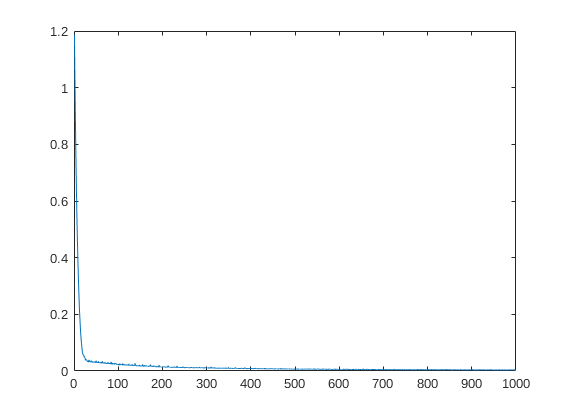
\includegraphics[width=\textwidth]{eta-polyak}
        \caption{Difference between $f(x_t)$ and $f^{opt}$ at each iteration using a Polyak step size.}
      \end{figure}

      \begin{figure}[H]
        \centering
          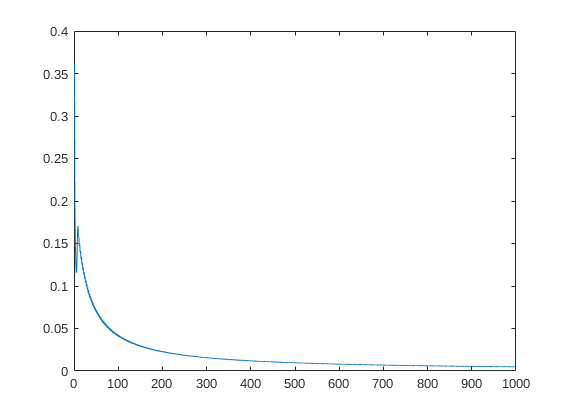
\includegraphics[width=\textwidth]{eta-t}
        \caption{Difference between $f(x_t)$ and $f^{opt}$ at each iteration using a $1/t$ step size. Note the slower convergence.}
      \end{figure}

      \begin{figure}[H]
        \centering
          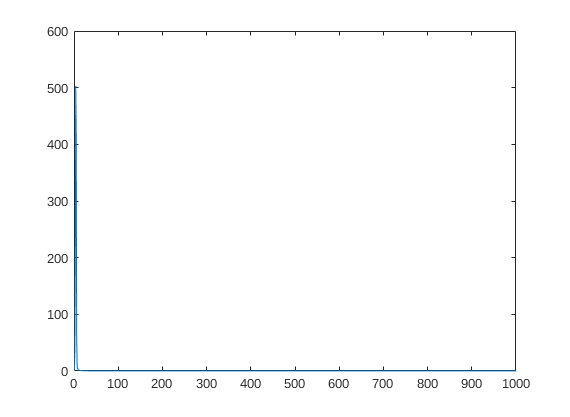
\includegraphics[width=\textwidth]{eta-t2}
        \caption{Difference between $f(x_t)$ and $f^{opt}$ at each iteration using a $1/t^2$ step size. Note that divergence at the beggining when the step size is too big. The convergence is also much slower than the other two but the scale of the y-axis is too large to tell.}
      \end{figure}

      \textbf{Code:}

      \begin{lstlisting}[style=Matlab-editor, basicstyle=\scriptsize]
        clear;
        clc;

        n = 5; p = 3; q = 6;
        A = randn(p,q,n);
        B = randn(p,q);

        cvx_begin
            variable x(n)    
            minimize( norm(A(:,:,1)*x(1)+A(:,:,2)*x(2)+A(:,:,3)*x(3)+A(:,:,4)*x(4)+A(:,:,5)*x(5) - B, 2) )
        cvx_end


        f_opt = cvx_optval;

        % Subgradient method, no need to project as we are in R^n
        T = 1000;
        y = zeros(T,5);
        g = zeros(T,5);
        f = zeros(T,1);
        tmp = zeros(6,6);

        for t = 1:T
            inner_mat = A(:,:,1)*y(t,1)+A(:,:,2)*y(t,2)+A(:,:,3)*y(t,3)+A(:,:,4)*y(t,4)+A(:,:,5)*y(t,5) - B;
            f(t) = norm(inner_mat, 2);
            [U,S,V] = svds(inner_mat, 1);
            
            % Calculate subgradient
            for i = 1:n
                tmp = 2*y(t,i)*A(:,:,i)'*A(:,:,i);
                
                for j = 1:n
                    if j ~= i
                        tmp = tmp + y(t,j)*A(:,:,i)'*A(:,:,j) + y(t,j)*A(:,:,j)'*A(:,:,i);
                    end
                end
                
                tmp = tmp - A(:,:,i)'*B - B'*A(:,:,i);
                g(t,i) = V'*tmp*V;
            end
           
            eta = (f(t)-f_opt)/(norm(g(t,:),2)^2);
            %eta = 1/t^2;
            %eta = 1/(t+30);
            y(t+1,:) = y(t,:) - eta*g(t,:);
        end

        plot(f-f_opt)
        f(T)-f_opt
      \end{lstlisting}

  \end{enumerate}

\end{answer}

\clearpage

\begin{exercise}
  \textbf{Step sizes that guarantee moving closer to the optimal set:} Consider the subgradient method iteration $\bm{x}^+ = \bm{x} - \eta \bm{g}$, where $\bm{g} \in \partial f(\bm{x})$. Let $f^*$ be the optimal objective value. Show that if $\eta < \frac{2(f(\bm{x}) - f^*)}{\lVert \bm{g} \rVert_2^2}$ (which is twice Polyak's optimal step size value) we have

  \begin{gather*}
    \lVert \bm{x}^+ - \bm{x}^* \rVert_2 < \lVert \bm{x} - \bm{x}^* \rVert_2
  \end{gather*}

  \noindent for any optimal point $\bm{x}^*$.

  \textbf{Remark:} Methods in which successive iterates move closer to the optimal set are called \textit{Fejer monotone}. Thus, the subgradient method, with Polyak's optimal step size, is \textit{Fejer monotone}.

\end{exercise}

\begin{answer}
  \

  The proof follows immediately using the majorizing function presented by Lemma 4.1 in the notes. We have by the lemma:

  \begin{gather*}
    \lVert \bm{x}^+ - \bm{x}^* \rVert_2^2 \leq \lVert \bm{x} - \bm{x}^* \rVert_2^2 - 2 \eta (f(\bm{x}) - f^*) + \eta^2 \lVert \bm{g} \rVert_2^2
  \end{gather*}

  \noindent If we wish to have the result that $\lVert \bm{x}^+ - \bm{x}^* \rVert_2 < \lVert \bm{x} - \bm{x}^* \rVert_2$, then we must have that

  \begin{gather*}
    - 2 \eta (f(\bm{x}) - f^*) + \eta^2 \lVert \bm{g} \rVert_2^2 < 0
  \end{gather*}

  \noindent Simple rearranging of this yields

  \begin{gather*}
    \eta < \frac{2(f(\bm{x}) - f^*)}{\lVert \bm{g} \rVert_2^2}
  \end{gather*}

  \noindent Note that dividing by $\eta$ is justified as if $\eta = 0$ then we are at the optimal point.

\end{answer}

\clearpage

\begin{exercise}
  \textbf{Gradient of squared distance (bonus):} Define the Euclidean projection onto a closed convex set $\mathcal{C}$ as

  \begin{gather*}
    \mathcal{P}_\mathcal{C}(\bm{x}) := \argmin_{\bm{z} \in \mathcal{C}} \lVert \bm{z} - \bm{x} \rVert_2
  \end{gather*}

  \noindent and let

  \begin{gather*}
    \text{dist}_\mathcal{C} (\bm{x}) :=\lVert \bm{x} - \mathcal{P}_\mathcal{C} (\bm{x}) \rVert_2
  \end{gather*}

  \noindent Show that the gradient of the squared distance $f(\bm{x}) := \frac{1}{2} \text{dist}_\mathcal{C}^2 (\bm{x})$ is

  \begin{gather*}
    \nabla f(\bm{x}) = \bm{x} - \mathcal{P}_\mathcal{C} (\bm{x})
  \end{gather*}

  \noindent Here, you can assume (without proof) that $f(\bm{x})$ is convex.

\end{exercise}

\begin{answer}
  \

  For conciseness, we use the the shorthand notation $\mathcal{P}_\mathcal{C}(\bm{x}) = \mathcal{P}_{\bm{x}}$. To show that the $\bm{x} - \mathcal{P}_{\bm{x}}$ is the gradient of $f(\bm{x})$ we must show

  \begin{gather*}
    f(\bm{y}) - f(\bm{x}) \geq (\bm{y} - \bm{x})^T (\bm{x} - \mathcal{P}_{\bm{x}})
  \end{gather*}

  Plugging in the definitions into the above

  \begin{gather*}
    \lVert \bm{y} - \mathcal{P}_{\bm{y}} \rVert_2^2 - \lVert \bm{x} - \mathcal{P}_{\bm{x}} \rVert_2^2  \geq 2(\bm{y} - \bm{x})^T (\bm{x} - \mathcal{P}_{\bm{x}})
  \end{gather*}

  Now we introduce some terms to the RHS and simplify

  \begin{gather*}
    \lVert \bm{y} - \mathcal{P}_{\bm{y}} \rVert_2^2 - \lVert \bm{x} - \mathcal{P}_{\bm{x}} \rVert_2^2  \geq 2(\bm{y} - \mathcal{P}_{\bm{y}} + \mathcal{P}_{\bm{y}} - \bm{x})^T (\bm{x} - \mathcal{P}_{\bm{x}}) \\
    \lVert \bm{y} - \mathcal{P}_{\bm{y}} \rVert_2^2 - \lVert \bm{x} - \mathcal{P}_{\bm{x}} \rVert_2^2  \geq 2(\bm{y} - \mathcal{P}_{\bm{y}})^T (\bm{x} - \mathcal{P}_{\bm{x}}) + 2(\mathcal{P}_{\bm{y}} - \bm{x})^T (\bm{x} - \mathcal{P}_{\bm{x}}) \\
    \lVert \bm{y} - \mathcal{P}_{\bm{y}} \rVert_2^2 + \lVert \bm{x} - \mathcal{P}_{\bm{x}} \rVert_2^2 - 2(\bm{y} - \mathcal{P}_{\bm{y}})^T (\bm{x} - \mathcal{P}_{\bm{x}})  \geq 2(\mathcal{P}_{\bm{y}} - \bm{x})^T (\bm{x} - \mathcal{P}_{\bm{x}}) + 2 \lVert \bm{x} - \mathcal{P}_{\bm{x}} \rVert_2^2 \\
    \lVert \bm{y} - \mathcal{P}_{\bm{y}} - \bm{x} + \mathcal{P}_{\bm{x}} \rVert_2^2 \geq 2(\mathcal{P}_{\bm{y}} - \bm{x})^T (\bm{x} - \mathcal{P}_{\bm{x}}) + 2 \lVert \bm{x} - \mathcal{P}_{\bm{x}} \rVert_2^2
  \end{gather*}

  Now, we expand the norm on the LHS differently

  \begin{gather*}
    \lVert \bm{y} - \bm{x} \rVert_2^2 +2(\bm{y} - \bm{x})^T (\mathcal{P}_{\bm{x}} - \mathcal{P}_{\bm{y}}) + \lVert \mathcal{P}_{\bm{x}} - \mathcal{P}_{\bm{y}} \rVert_2^2  \geq 2(\mathcal{P}_{\bm{y}} - \bm{x})^T (\bm{x} - \mathcal{P}_{\bm{x}}) + 2 \lVert \bm{x} - \mathcal{P}_{\bm{x}} \rVert_2^2
  \end{gather*}

  Using the non-expansiveness property of projections, we can upper bound the LHS

  \begin{gather*}
    2 \lVert \bm{y} - \bm{x} \rVert_2^2 +2(\bm{y} - \bm{x})^T (\mathcal{P}_{\bm{x}} - \mathcal{P}_{\bm{y}}) \geq 2(\mathcal{P}_{\bm{y}} - \bm{x})^T (\bm{x} - \mathcal{P}_{\bm{x}}) + 2 \lVert \bm{x} - \mathcal{P}_{\bm{x}} \rVert_2^2
  \end{gather*}

  Simplifying this expression

  \begin{gather*}
    \lVert \bm{y} - \bm{x} \rVert_2^2 +(\bm{y} - \bm{x})^T (\mathcal{P}_{\bm{x}} - \mathcal{P}_{\bm{y}}) \geq (\mathcal{P}_{\bm{y}} - \mathcal{P}_{\bm{x}})^T (\bm{x} - \mathcal{P}_{\bm{x}}) \\
    \lVert \bm{y} - \bm{x} \rVert_2^2 \geq (\mathcal{P}_{\bm{y}} - \mathcal{P}_{\bm{x}})^T (\bm{x} - \mathcal{P}_{\bm{x}} + \bm{y} - \bm{x}) \\
    \lVert \bm{y} - \bm{x} \rVert_2^2 \geq (\mathcal{P}_{\bm{y}} - \mathcal{P}_{\bm{x}})^T (\bm{y} - \mathcal{P}_{\bm{x}})
  \end{gather*}

  Introducing $\mathcal{P}_{\bm{y}} - \mathcal{P}_{\bm{y}}$ to the inner product of the RHS yields

  \begin{gather*}
    \lVert \bm{y} - \bm{x} \rVert_2^2 \geq \lVert \mathcal{P}_{\bm{y}} - \mathcal{P}_{\bm{x}} \rVert_2^2 + (\mathcal{P}_{\bm{y}} - \mathcal{P}_{\bm{x}})^T (\bm{y} - \mathcal{P}_{\bm{y}})
  \end{gather*}

  Now, we note that the second term in the RHS $(\mathcal{P}_{\bm{y}} - \mathcal{P}_{\bm{x}})^T (\bm{y} - \mathcal{P}_{\bm{y}}) \geq 0$ by the convexity of $\mathcal{C}$. To see this, note that $\bm{y} - \mathcal{P}_{\bm{y}}$ is perpendicular to the tangent at $\mathcal{P}_{\bm{y}}$ and that $\mathcal{P}_{\bm{x}}$ and $\mathcal{P}_{\bm{y}}$ are contained inside $\mathcal{C}$ and so these two vectors must have a positive inner product. Thus, we can lower bound the LHS by dropping this term

  \begin{gather*}
    \lVert \bm{y} - \bm{x} \rVert_2^2 \geq \lVert \mathcal{P}_{\bm{y}} - \mathcal{P}_{\bm{x}} \rVert_2^2
  \end{gather*}

  Which is our non-expansiveness property that we know is true. Thus, our original inequality must be true and we conclude that

  \begin{gather*}
    \nabla f(\bm{x}) = \bm{x} - \mathcal{P}_\mathcal{C} (\bm{x})
  \end{gather*}

\end{answer}

\end{document}